\section{Machine Learning Principles} \label{sec:ml_contextualization}

\Acf{ML} is a subfield of Computer Science that focuses on developing algorithms and models that enable computers to learn from data and make predictions or decisions without being explicitly programmed for each specific task \citep{goodfellow2016deep}. Unlike traditional programming (see Figure \ref{fig:traditional_programming_pipeline}), which follows strict rules, \ac{ML} systems (see Figure \ref{fig:machine_learning_pipeline}) identify patterns in data and adjust their parameters to improve their performance over time. The concern then shifts from ``How do I program the computer to perform a task?'' to ``How do I create models that learn from the data and how do I evaluate them?''

\begin{figure}[!ht]
  \centering
  \caption{Visual comparison between Classical Programming and Machine Learning.}
  \begin{subfigure}[c]{0.48\columnwidth} % Reduced width
    \centering
    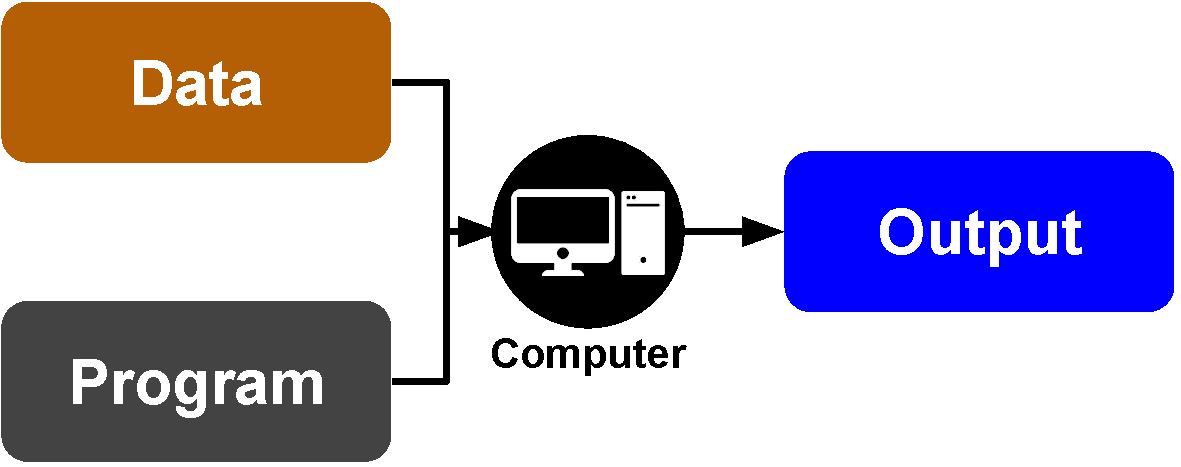
\includegraphics[width=\currprop]{figures/3_theoretical_background/shallow_learning/traditional_programming_pipeline.pdf} % + 0.19
    \caption{}
    \label{fig:traditional_programming_pipeline}
  \end{subfigure}
  \hfil % This provides the horizontal space
  \begin{subfigure}[c]{0.48\columnwidth} % Reduced width
    \centering
    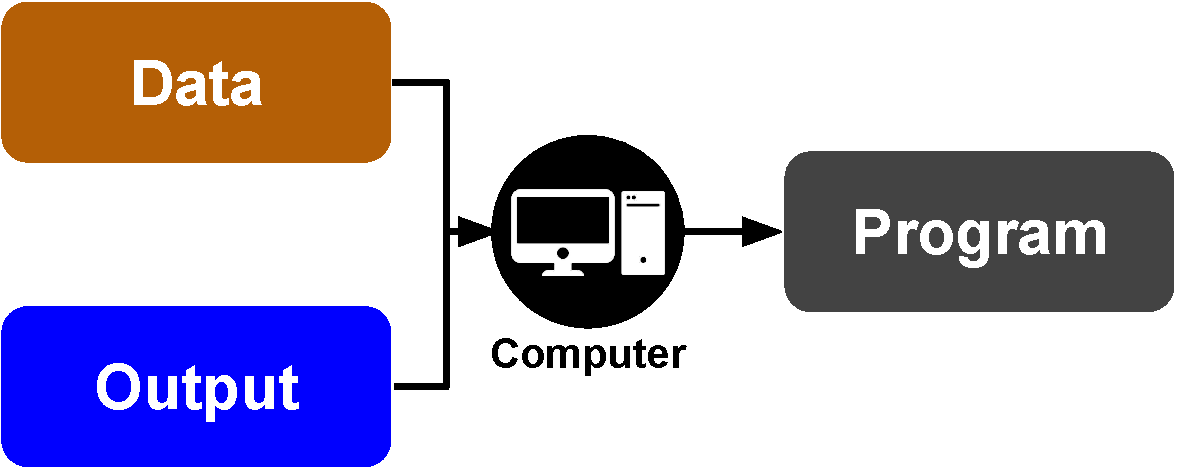
\includegraphics[clip,width=\currprop]{figures/3_theoretical_background/shallow_learning/machine_learning_pipeline.pdf}
    \caption{}
    \label{fig:machine_learning_pipeline}
  \end{subfigure}

  \fignote{(a) shows Classical Programming paradigm, while (b) shows the new Machine Learning paradigm.}
\end{figure}

\subsection{Shallow Learning models}

In this context, \ac{SL} is a \ac{ML} approach that works well for tabular data, but requires preprocessing steps for unstructured data (such as images, videos, texts, or \ac{SITS}) converting them into tabular data, a complete subfield called Feature Engineering \cite{zheng2018feature}. In addition to the requirement for handcrafted features, such models are generally older and less complex compared to current models, and the name ``shallow'' contrasts with \ac{DL}, which will be explained in more detail in Section \ref{sec:deep_learning}. Also, \ac{SL} models often require less data for training and are faster to train and implement, as well as being more interpretable, which makes it easier to understand how decisions are made by the model. However, to use them, it is necessary to choose those handcrafted features (extraction and selection), which can be challenging, especially in areas such as \ac{CV} and \ac{RS}.

\subsubsection{K-Nearest Neighbor (KNN)}

\acf{KNN} is an \ac{SL} classification model based on the principle that similar instances in a dataset tend to be located close to each other in the feature space space \citep{cover1967nearest}. Unlike other models that construct an explicit mathematical function during training, \ac{KNN} is classified as a lazy learner, as it does not generate a discriminative model in advance; instead, it stores the entire training dataset and postpones computational processing until the moment of inference. 

The algorithm's operation is based on calculating the distance between the sample to be classified and all examples in the training set -- usually the Euclidean distance, although other metrics such as Manhattan or Minkowski can be applied. The model selects the $K$ closest neighbors and defines the class of the new object by majority vote (see Figure \ref{fig:knn}). In the context of regression, \ac{KNN} estimates the output value using the arithmetic or weighted average of the values of the $K$ neighbors. However, its computational search cost increases linearly with the number of samples ($O(n)$) and is highly sensitive to the scale of the variables, requiring normalization steps and, often, dimensionality reduction techniques (such as PCA).

\begin{figure}[ht!]
    \centering
    \caption{Diagram of a K-nearest neighbor model.}
    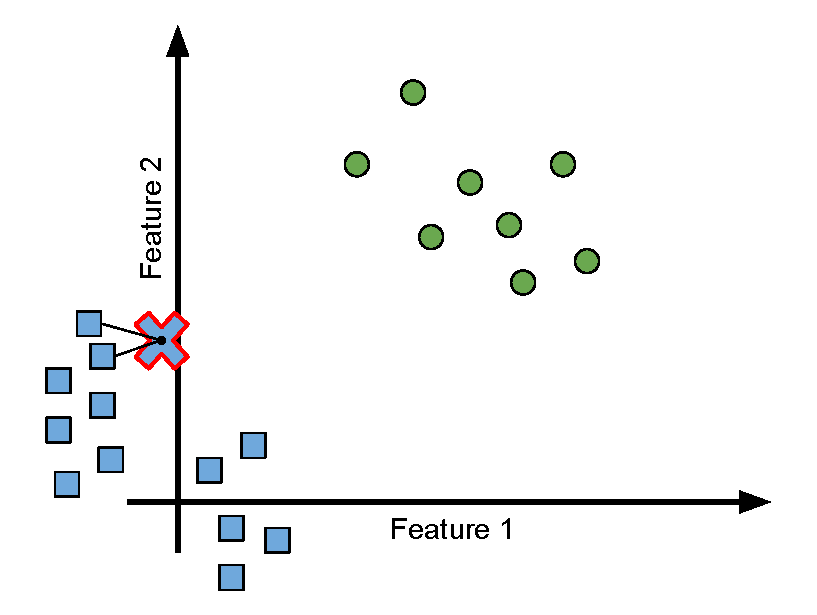
\includegraphics[width=.7\linewidth]{figures/3_theoretical_background/shallow_learning/knn.pdf}
    \fignote{One should notice that, in this model K=2 so, when a prediction sample is given (the X in the figure), the two most near training samples classes are verified, than their class will be assigned to the given prediction sample.}
    \label{fig:knn}
\end{figure}

\Ac{KNN} is widely used as a test for \ac{SSL} pre-training due to its simplicity and ability to provide a quick assessment of the quality of the generated embeddings, being retrained at each new pre-training epoch.

\subsubsection{Support Vector Machine (SVM)}

\Acf{SVM} is a widely used supervised learning algorithm for classification and regression tasks \citep{boser1992training}. SVM works by finding the optimal hyperplane that separates different classes of data in feature space, maximizing the margin between classes (see the Figure \ref{fig:svm}). In cases where the data is not linearly separable (such as spectral bands in \ac{RS}), \ac{SVM} can use the ``kernel trick'' to transform the data into a higher-dimensional space where linear separation is possible. \ac{SVM} is known for its effectiveness on high-dimensional datasets and its robustness against overfitting, especially when configured with the correct parameters.

\begin{figure}[ht!]
    \centering
    \caption{Diagram of a Support Vector Machine model.}
    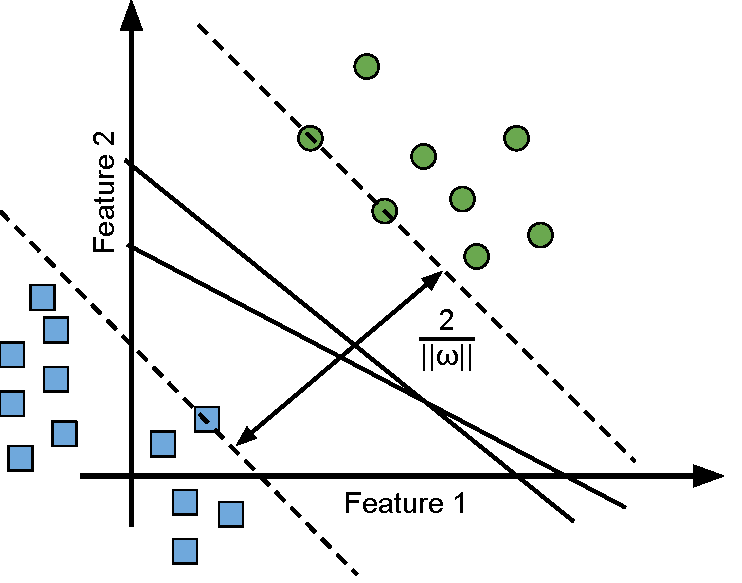
\includegraphics[width=.7\linewidth]{figures/3_theoretical_background/shallow_learning/svm.pdf}
    \label{fig:svm}
\end{figure}

The main idea behind the kernel trick is to map the input data to a higher-dimensional space where linear separation between classes can be achieved. Instead of explicitly calculating the coordinates of the data in this higher-dimensional space, the kernel trick allows us to directly calculate the inner products between the data vectors in the original space using specific kernel functions. The most common kernels include the Linear Kernel (for data that is already linearly separable), the Polynomial Kernel (which introduces curvature), and, notably, the Radial Basis Function (RBF) Kernel, which is one of the most widely used due to its effectiveness in dealing with complex separations in \ac{RS}.

Despite its theoretical robustness and good performance on many datasets, \ac{SVM} presents some practical challenges. First, the high computational cost and training time can be significant, especially with increasing data volume (very large datasets, such as pixels of multiespectral satellite images). Training time generally scales between $O(n^2)$ and $O(n^3)$ (where $n$ is the number of training samples), making it less efficient for large volumes of raw data than, for example, \ac{RF}. Second, \ac{SVM} performance is highly sensitive to the choice and adjustment of Kernel parameters (hyperparameters) and the penalty parameter ($C$). As such, \ac{SVM} usually requires several different long training sessions (with different hyperparameters), making the model quite costly.

\subsubsection{Random Forest (RF)}
\label{sec:rf}

\Acf{RF} is a \ac{SL} model that combines multiple simpler models, \acf{DT}, to improve the quality and robustness of predictions \citep{breiman2001random}. A \ac{DT} (see the black bounding box in Figure \ref{fig:random_forest}) works by recursively dividing a dataset into smaller, more homogeneous subsets based on input characteristics (variables) \citep{quinlan1986induction}. Although simple and interpretable, a single \ac{DT} is often susceptible to overfitting, which means that it may perform well on training data but poorly on test data. However, on the plus side, it is one of the most interpretable models in the entire field of machine learning, precisely because it approximates the way humans think about tasks or define classes, as exemplified above.

\begin{figure}[ht!]
    \centering
    \caption{Diagram of a Random Forest model.}
    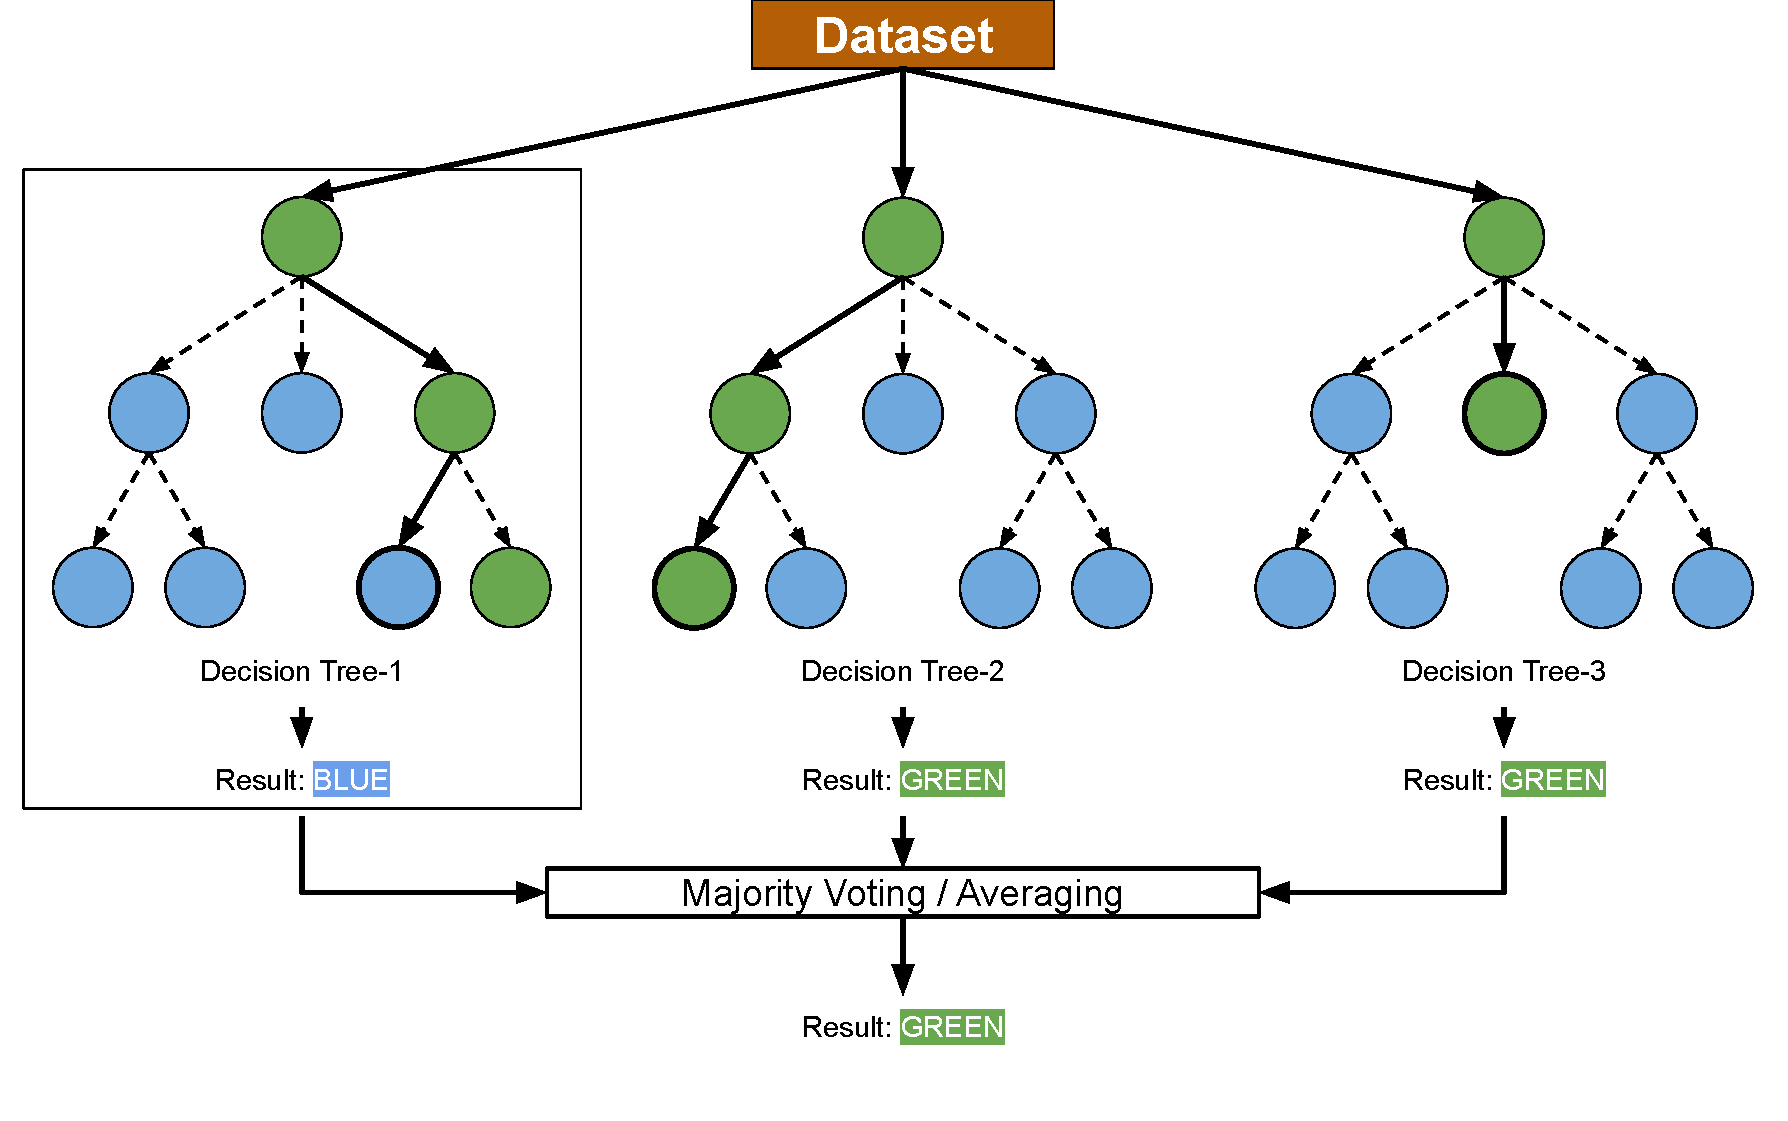
\includegraphics[width=1\linewidth]{figures/3_theoretical_background/shallow_learning/random_forest.pdf}
    \fignote{The black bounding box is highlighting a decision tree, the core subpart of a RF.}
    \label{fig:random_forest}
\end{figure}

In \ac{RS}, \ac{RF} is a classification tool that is still widely used today, mainly for \ac{LULC}. It is widely used because it does not require data preprocessing, being one of the few models that is robust to data scale. Thus, it is quite common to classify image pixels or satellite mosaics, creating thematic maps in shallow semantic segmentation. Due to its training speed and lack of preprocessing requirements, it is also a widely used model as a baseline for more advanced techniques.

\subsubsection{Gradient Boosting (GB)}

\Acf{GB} models, on the other hand, are very similar to \ac{RF} (see Section \ref{sec:rf}), as they also build multiple \ac{DT} to improve predictive performance \citep{friedman2001greedy}. However, while \ac{RF} builds trees independently and joins them together, \ac{GB} builds trees sequentially, where each new tree attempts to correct the errors of the previous trees. This process is known as boosting, and the goal is to minimize a specific loss function by iteratively adding weak models that improve the overall performance of the model.

\begin{figure}[ht!]
    \centering
    \caption{Diagram of a Gradient Boosting (GB) model.}
    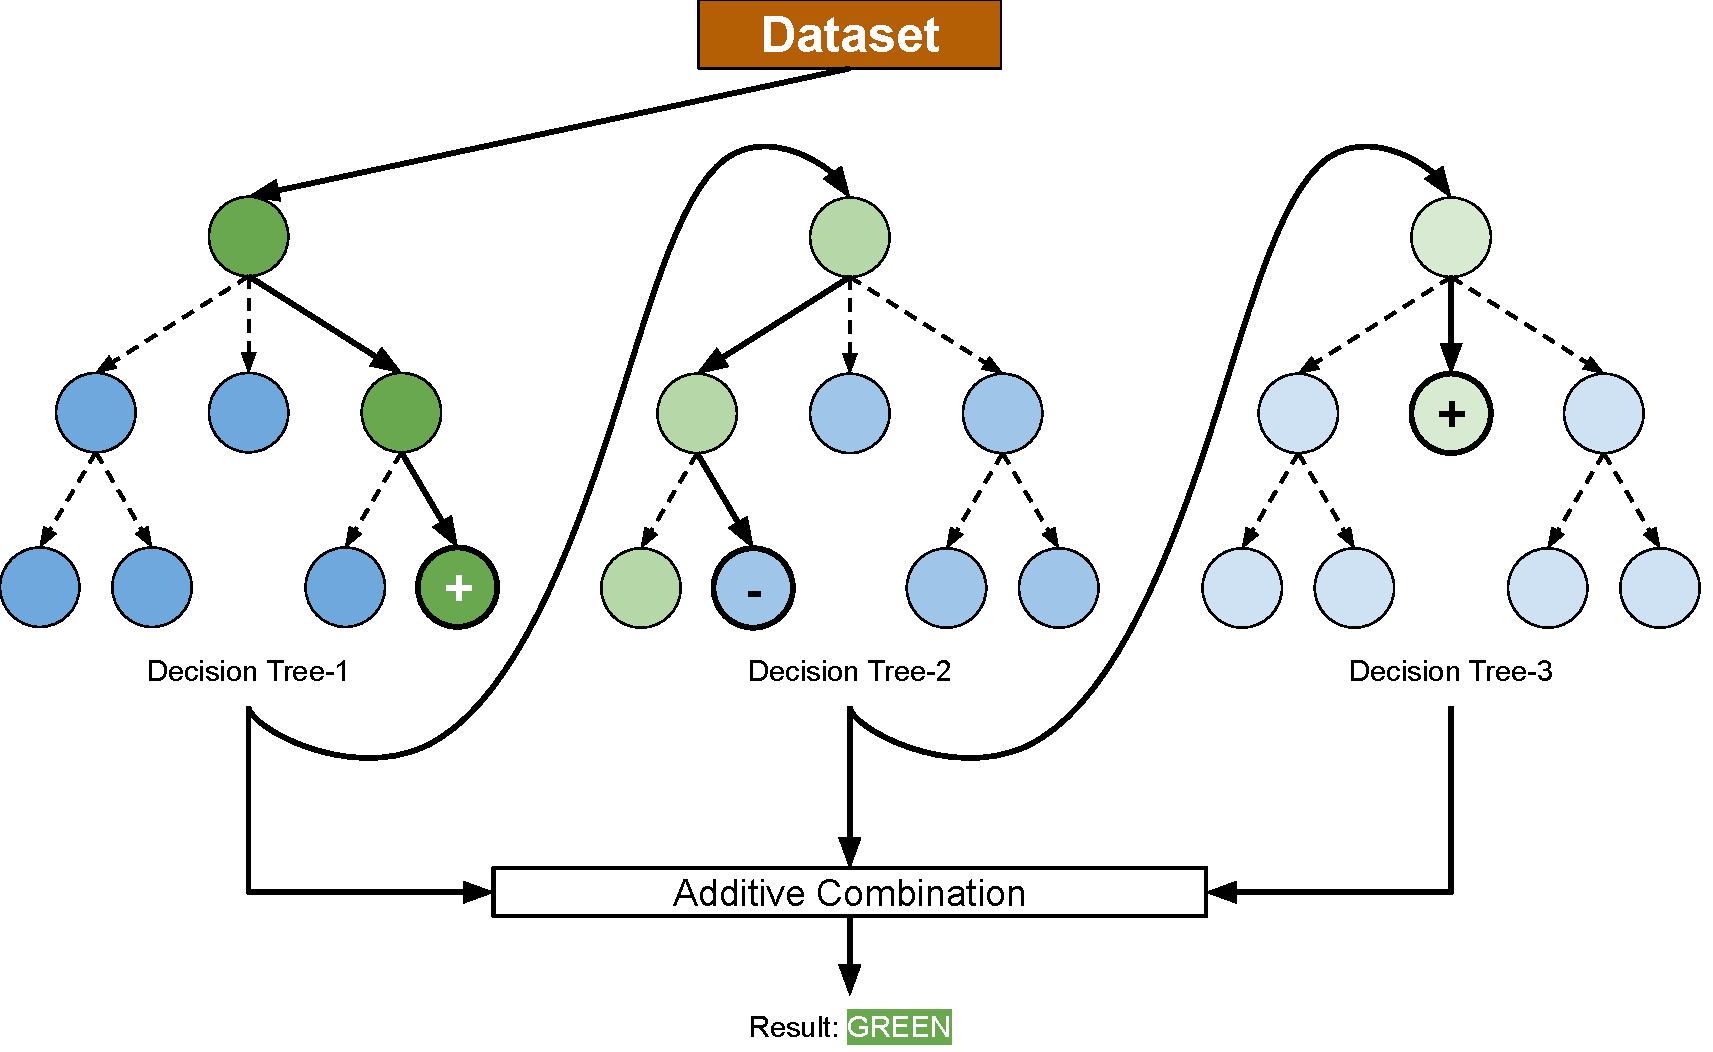
\includegraphics[width=1\linewidth]{figures/3_theoretical_background/shallow_learning/gradient_boosting.pdf}
    \fignote{One should notice that the Decision Trees refine each other's decisions.}
    \label{fig:gradient_boosting}
\end{figure}

In \ac{RS}, \ac{GB} has uses that are extremely similar to RF, functioning as a more costly
alternative - both in terms of computational cost and scientist time - but ofter with better results. Two famous implementations of \ac{GB} stand out: XGBoost and LightGBM. The main difference in standard hyperparameter optimization strategies between LightGBM and XGBoost lies in the treatment of the tree: LightGBM uses depth-based (leaf-wise) tree growth, generally resulting in deeper and more asymmetric \ac{DT} by default, while XGBoost typically uses level-wise growth, producing balanced \ac{DT}, which directly affects the standard parameters of maximum depth and number of leaves, both of which are widely used in \ac{RS}.

\subsubsection{Multi-Layer Perceptron (MLP)}
\label{sec:mlp}

The \ac{MLP} is a classic Artificial Neural Network (ANN) architecture consisting of multiple layers of fully connected neurons, i.e., each neuron in one layer is connected to all neurons in the next layer \citep{rosenblatt1958perceptron, rumelhart1986learning}. Such a model is also called a Feedforward Neural Network (FNN). The \ac{MLP} is composed of an input layer, one or more hidden layers, and an output layer. The hidden layers apply nonlinear activation functions, such as \ac{ReLU} or sigmoid, to introduce nonlinearity to the model.

\begin{figure}[ht!]
    \centering
    \caption{Diagram of a Multi-Layer Perceptron.}
    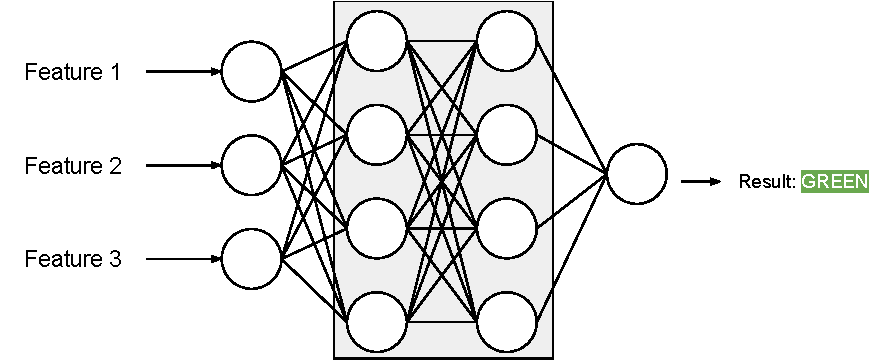
\includegraphics[width=.8\linewidth]{figures/3_theoretical_background/deep learning/mlp.pdf}
    \label{fig:mlp}
\end{figure}

Historically, \ac{MLP} represents the foundational architecture for \ac{DL} models. While deep configurations exist, simpler implementations with few hidden layers are often categorized alongside shallow methods. Today, \acs{MLP}s are still used at the end of other more complex neural networks to perform the final step of mapping the extracted features to the desired classes or output values. Also, this model is often used as baselines.

\subsubsection{K-Means}

K-Means is possibly the best known and most widely used Unsupervised \ac{SL} model \citep{macqueen1965some, lloyd1982least}. Unsupervised Learning is a \ac{ML} technique where the model is trained using an unlabeled dataset, i.e., the input examples do not have associated desired outputs. The goal of the model is to identify patterns, structures, or clusters in the data without the guidance of predefined labels. K-Means is a clustering algorithm that aims to partition a data set into K distinct groups, where each group is represented by a centroid. The algorithm works iteratively, assigning each data point to the nearest centroid and then recalculating the centroids based on the new assignments. This process continues until the assignments of the data points no longer change significantly or until a maximum number of iterations is reached.

\begin{figure}[ht!]
    \centering
    \caption{The impact of applying K-Means in a Unlabeled Dataset.}
    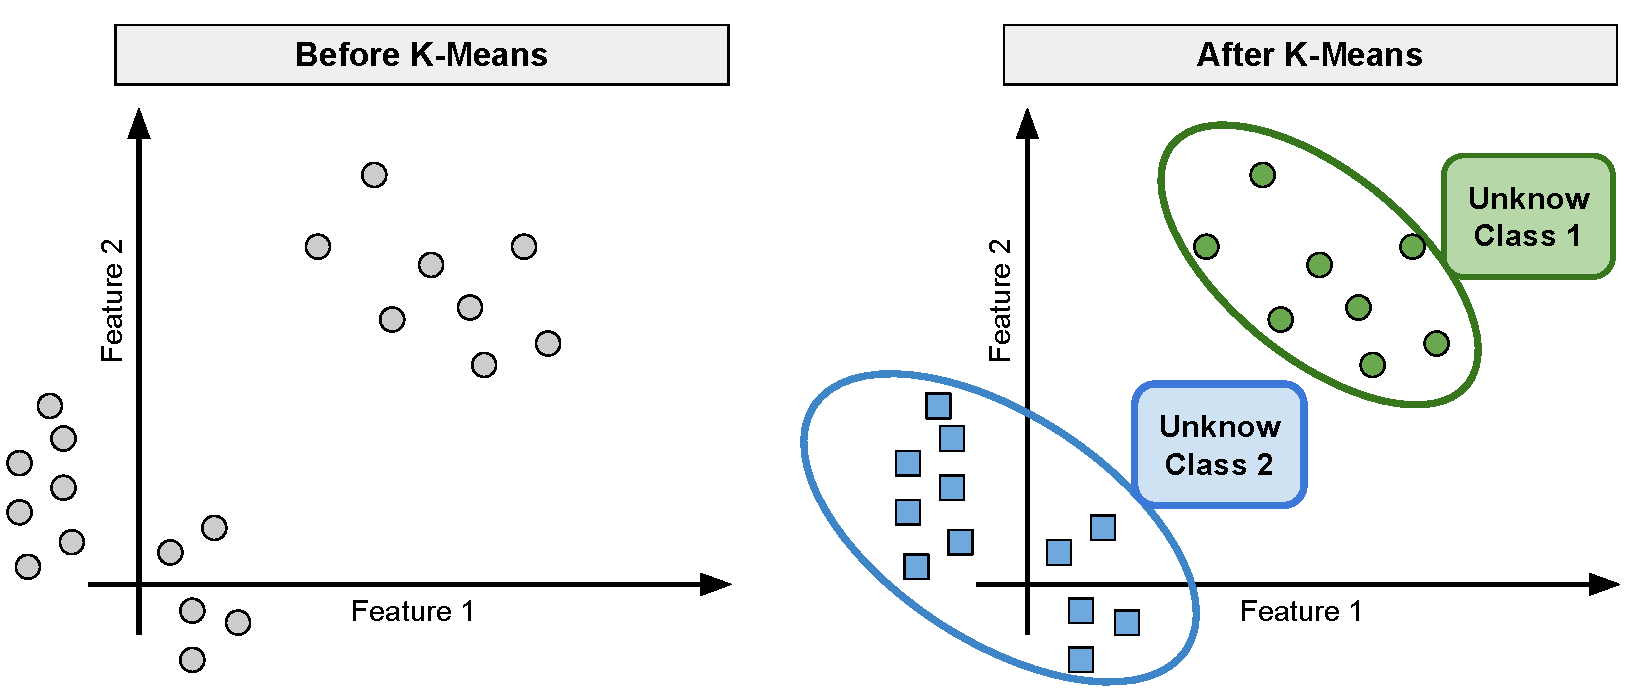
\includegraphics[width=1\linewidth]{figures/3_theoretical_background/shallow_learning/kmeans.pdf}
    \label{fig:kmeans}
\end{figure}

The big challenge is to define the value of $K$, which can be done using methods such as the elbow method or silhouette score. In \ac{RS}, K-Means is often used for image segmentation, where the goal is to group pixels with similar spectral characteristics, facilitating the identification of different types of \ac{LULC}, serving both to facilitate exploratory analysis and to assist in subsequent supervised classification tasks.

\subsubsection{Gaussian Mixture Model (GMM)}

The \acf{GMM} is an \ac{SL} unsupervised model that assumes that all data points are generated from a mixture of a finite number of Gaussian distributions with unknown parameters \citep{dempster1977maximum}. While K-Means performs hard clustering, where each point belongs exclusively to a centroid/cluster, \ac{GMM} performs soft clustering, in which the model provides the probability of a given data point belonging to each of the clusters, allowing for a more robust handling of uncertainties and class overlaps.

The model is adjusted using the Expectation-Maximization (EM) algorithm. In the Expectation step, the algorithm estimates the probability of each point belonging to each Gaussian component; in the Maximization step, the Gaussian parameters (mean, covariance, and mixture weight) are updated to maximize the likelihood of the observed data. Also similar to K-Means, to use \ac{GMM} it is necessary to determine the number of components (clusters) to be used (see Figure \ref{fig:gmm}).

\begin{figure}[ht!]
    \centering
    \caption{Diagram of a Gaussian Mixture Model.}
    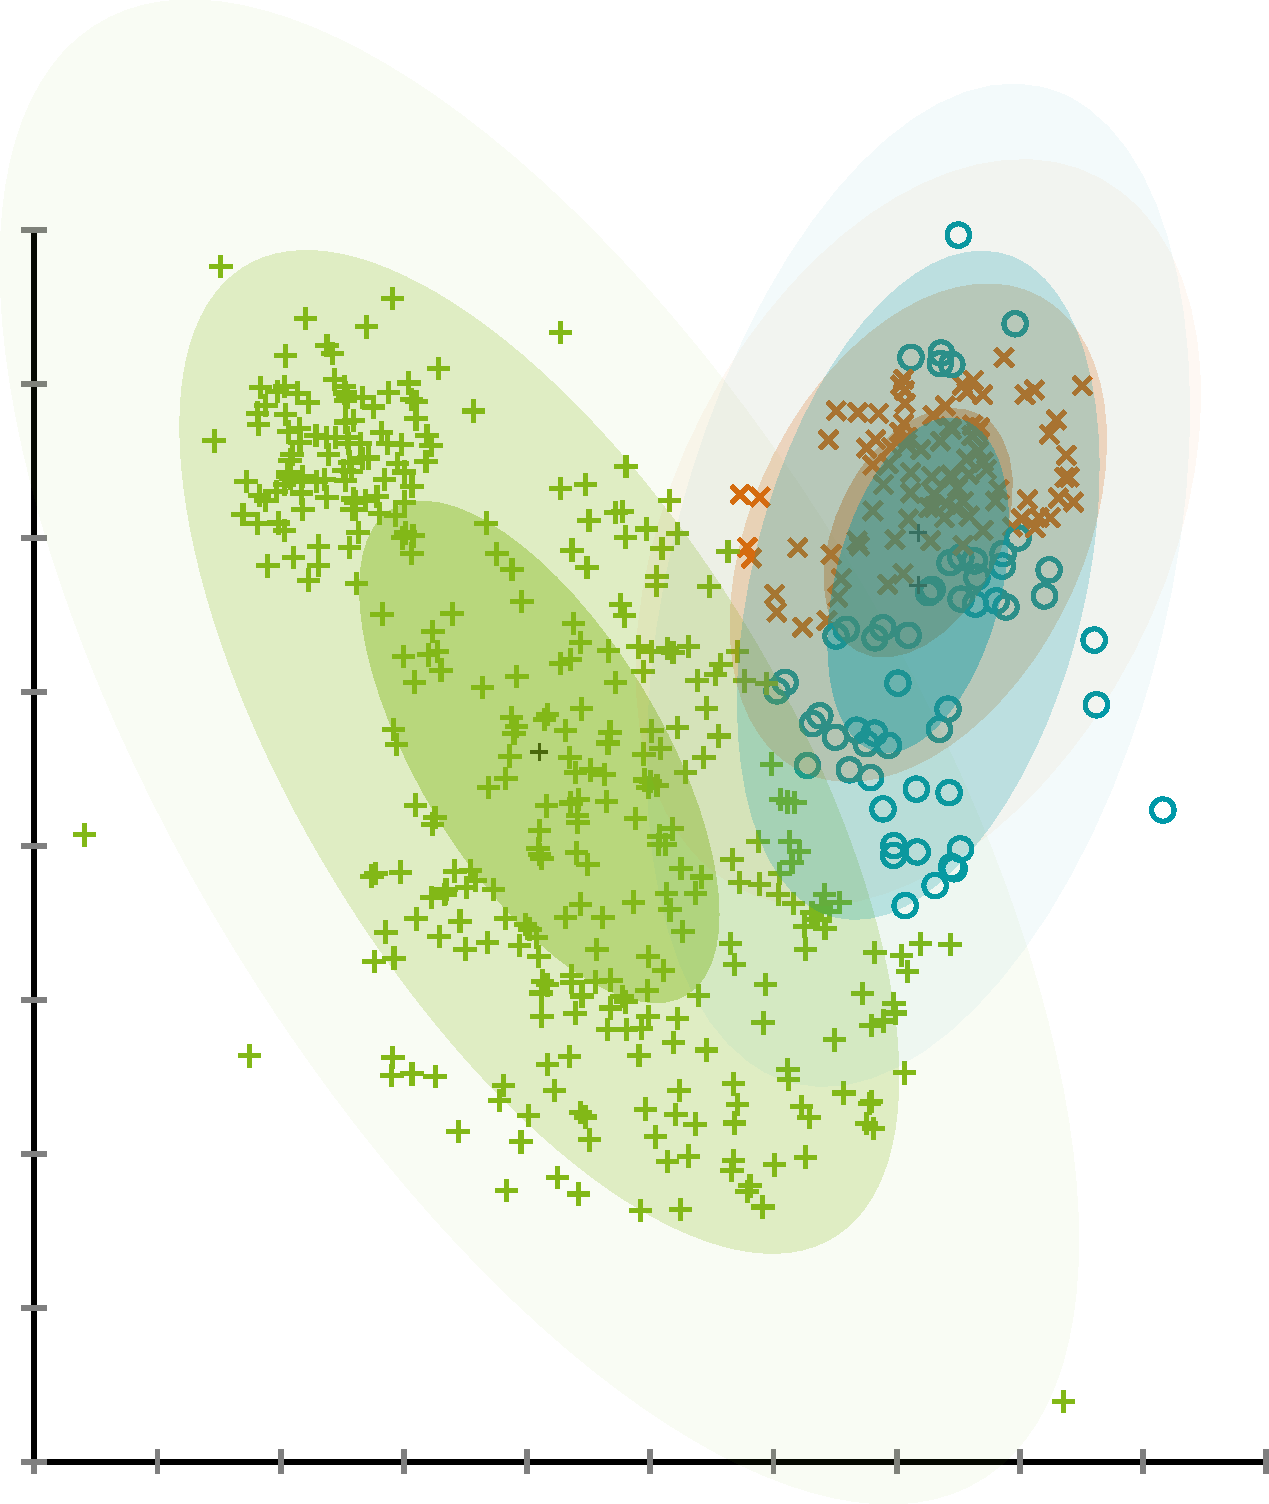
\includegraphics[width=.7\linewidth]{figures/3_theoretical_background/shallow_learning/gmm.pdf}
    \fignote{This example shows a GMM with number of components=3. Adapted from \href{https://dm.cs.tu-dortmund.de/mlbits/cluster-em-gmm-demo/}{TU Dortmund}}
    \label{fig:gmm}
\end{figure}


\subsection{Deep Learning models}
\label{sec:deep_learning}

On the other hand, \ac{DL} is a Machine Learning approach that uses latent data representations, meaning that the model itself learns to extract relevant features from raw data, eliminating the need for manual handcrafted feature extraction (with the exception, of course, of data normalization, which helps in model training convergence) \cite{bishop2023deep}. The best-known \ac{DL} models are Artificial Neural Networks (ANNs), which are composed of multiple layers of interconnected artificial neurons \cite{goodfellow2016deep}. Each neuron receives inputs, applies an activation function, and transmits the output to the neurons in the next layer. A loss function is defined to quantify the difference between the model's predictions and the actual values, and the model is trained using optimization algorithms, such as gradient descent, to adjust the weights of the connections between neurons in order to minimize this loss. In supervised learning, the most common loss functions include cross-entropy for classification and mean squared error for regression, which directly compare the model's predictions with the actual labels during training. Unsupervised techniques is also used in \ac{DL} to learn representations of data without explicit labels with different loss functions.

\subsubsection{Convolutional Neural Network (CNN)}
\label{sec:cnn}

A \ac{CNN} is a \ac{DL} model specially designed to process images \citep{lecun1989backpropagation}. \ac{CNN} are composed of convolutional layers that apply filters (or kernels) to extract local features from the input data, such as edges, textures, and spatial patterns. These layers are followed by pooling layers, which reduce the dimensionality of the data while retaining the most important features. Finally, an \ac{MLP} (see Section \ref{sec:mlp}) is generally used to perform classification or regression based on the extracted features.

\begin{figure}[ht!]
    \centering
    \caption{Diagram of a Convolutional Neural Network.}
    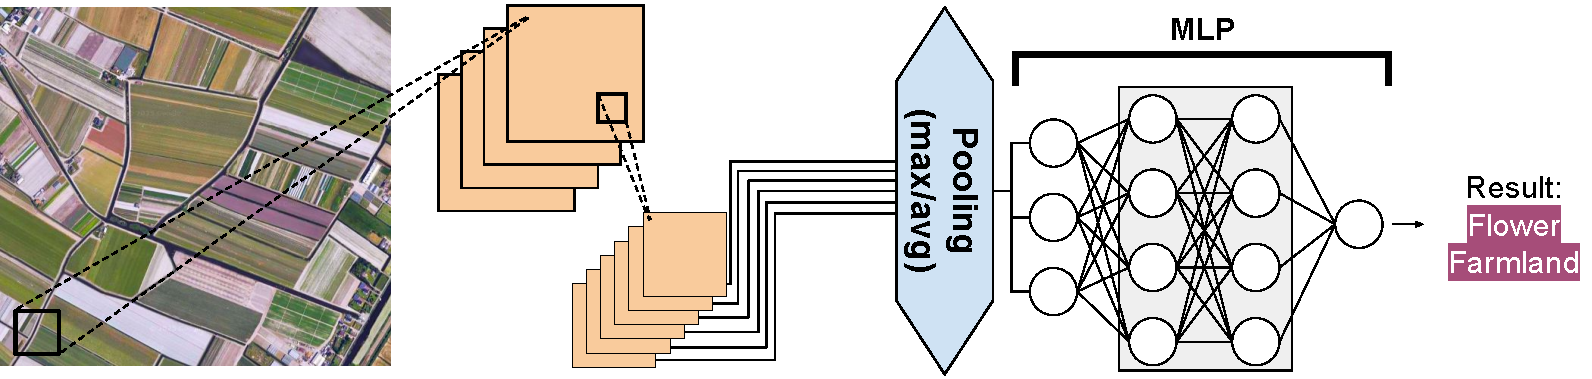
\includegraphics[width=1\linewidth]{figures/3_theoretical_background/deep learning/cnn.pdf}
    \label{fig:cnn}
\end{figure}

The motivation behind \ac{CNN} is to avoid the extremely high number of parameters that an \ac{MLP} would have when dealing with images, which generally have high dimensionality. For example, a $256\times256$ pixel Sentinel 2 image has $655360$ entries ($256 \times 256 \times 10$), which would result in millions of parameters in a typical \ac{MLP}. \acs{CNN}s allow kernels- such as Sobel and Canny kernels- to be trained and customized for each dataset, drastically reducing the number of parameters and making training possible.

The history of \acp{CNN} began with its use for character recognition \citep{lecun1989backpropagation} and the consolidation of LeNet-5 \citep{lecun2002gradient}, but it was AlexNet \citep{krizhevsky2012imagenet} that revolutionized the field by demonstrating the potential of GPUs -- which led to their widespread use throughout the field of machine learning -- and the \ac{ReLU} function in deep networks. This was followed by approaches such as VGG \citep{simonyan2014very}, focused on depth with small filters, and GoogleNet \citep{szegedy2015going}, which introduced Inception modules for multiscale processing, a technique refined in subsequent versions \citep{szegedy2016rethinking,szegedy2017inception}. A definitive milestone was ResNet \citep{he2016deep}, whose residual connections that dealt with Vanishing Gradients enabled networks with hundreds of layers, underpinning models such as ResNeXt \citep{xie2017aggregated}, based on cardinality, and DenseNet \citep{huang2017densely}, which prioritizes feature reuse (see Figure \ref{fig:cnn_hist}).

\begin{figure}[ht!]
    \centering
    \caption{Historical diagram of the evolution of Convolutional Neural Networs.}
    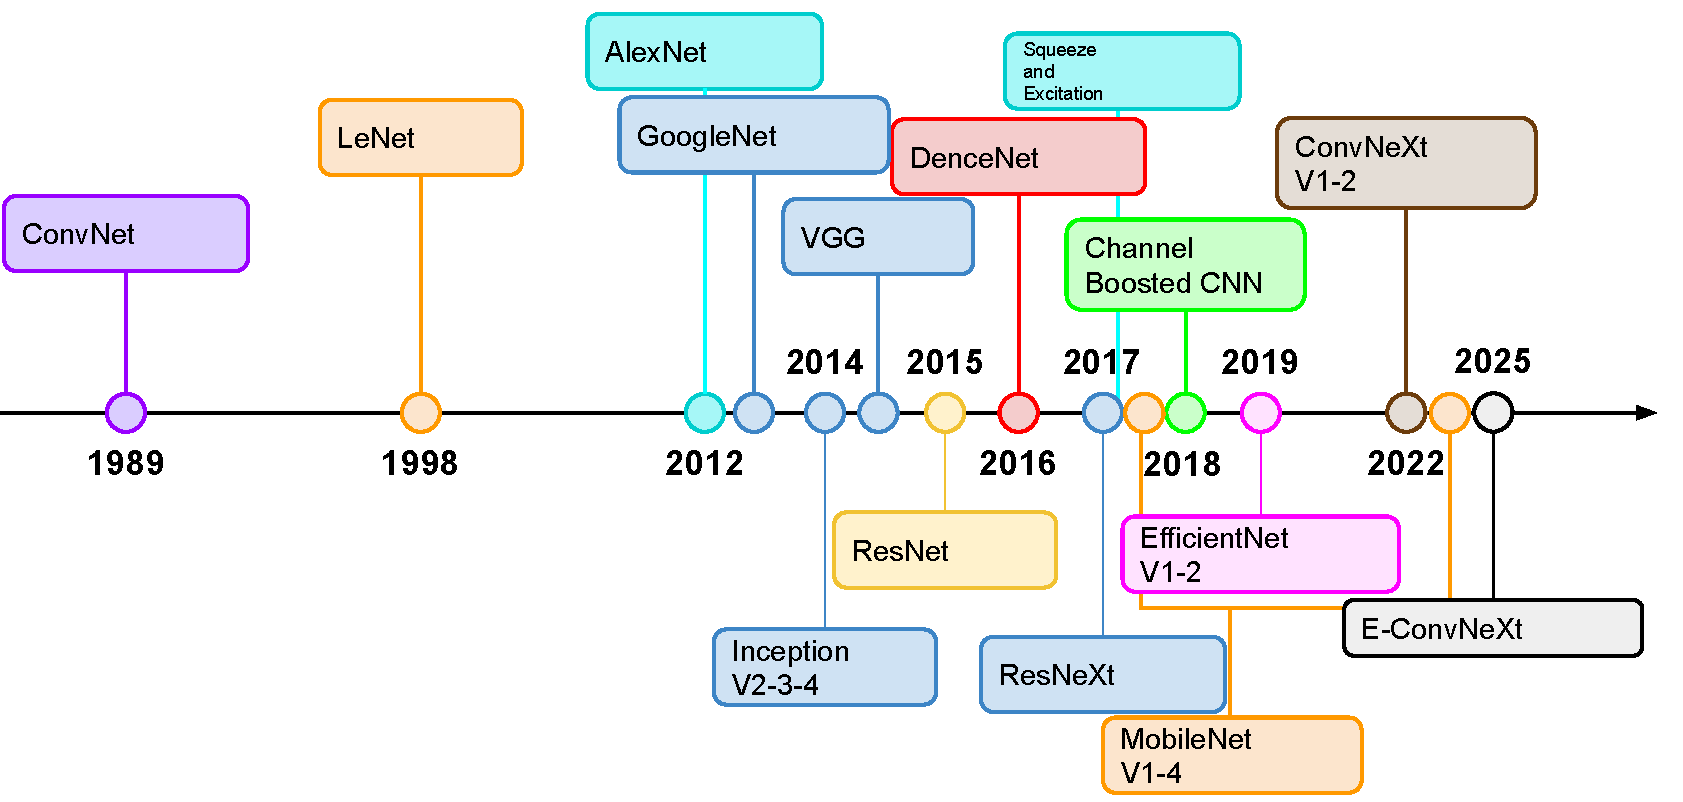
\includegraphics[width=1\linewidth]{figures/3_theoretical_background/deep learning/cnn_history.pdf}
    \label{fig:cnn_hist}
\end{figure}

Recently, efficiency has become the priority with the EfficientNet family \citep{tan2019efficientnet,tan2021efficientnetv2}, which optimized the width and depth scaling of networks. Being contemporary, the MobileNet series \citep{howard2017mobilenetsefficientconvolutionalneural,sandler2019mobilenetv2invertedresidualslinear,howard2019searchingmobilenetv3,qin2024mobilenetv4universalmodels} leveraged depthwise separable convolutions to balance latency and accuracy in resource-constrained environments. Concurrently, Squeeze-and-Excitation networks \citep{hu2019squeezeandexcitationnetworks} introduced channel-wise attention mechanisms to explicitly model interdependencies between channels, enhancing representational power with minimal computational overhead. In response to the rise of Transformers, the ConvNeXt architecture \citep{liu2022convnet} modernized \acp{CNN} with contemporary design choices, evolving to V2 \citep{woo2023convnext} with the use of masked autoencoders and to E-ConvNeXt \citep{wang2025convnext}, focused on low-resource devices. Complementarily, approaches such as Channel Boosted CNN \citep{khan2018new} explored channel diversity via transfer learning in an attempt to keep \acp{CNN} competitive in the face of new computer vision paradigms, especially in scenarios with low computational resources or little data.

\subsubsection{Semantic Segmentation Models}
\label{sec:fcn}

Some adaptions were done to convert \ac{CNN}s (see Section \ref{sec:cnn}) for semantic segmentation tasks, where the goal is to classify each pixel in an image into a specific class. One of the first adaptations, and still widely used today, is the \acf{FCN} \citep{long2015fully}. The strategy used was to replace the typical final \ac{MLP} of \ac{CNN} with deconvolution (or upsampling) layers, allowing the network to process images of any size and produce corresponding segmentation maps (see Figure \ref{fig:fcn}) .

\begin{figure}[ht!]
    \centering
    \caption{Diagram of a Fully Convolutional Network model.}
    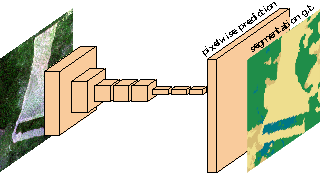
\includegraphics[width=.75\linewidth]{figures/3_theoretical_background/deep learning/fcn.pdf}
    \fignote{Adapted from Long et al \citep{long2015fullyconvolutionalnetworkssemantic}}
    \label{fig:fcn}
\end{figure}

This architecture is especially useful in \ac{RS} for LULC and Parcel Delineation applications -- as they are intrinsically semantic segmentation applications -- in addition to some uses in Crop Mapping or Crop Yielding. Furthermore, variations in which two \ac{FCN} are combined and have their embeddings concatenated are also used for Change Detection.

Aside from the FCN strategy, another common strategy for semantic segmentation networks is that of encoder-decoder networks, such as the U-Net model. U-Net was designed for biomedical image segmentation tasks, but is also possibly the most historically used \ac{DL} model in \ac{RS} \citep{ronneberger2015u}. The main innovation of U-Net is its ``U''-shaped structure, which consists of a path of reduced spatial resolution and increased number of channels (encoder) and subsequently a path of increased spatial resolution and decreased number of channels (decoder). The encoder follows a design pattern similar to that of \ac{CNN}, using blocks containing convolutional layers, \ac{ReLU} activation, and max pooling. On the other hand, the decoder is composed of upsampling and convolution layers, which help to reconstruct the spatial resolution of the image. This architecture allows the network to capture contexts of different scales while maintaining accurate spatial information. The Decision Factor of U-Net is the skip connections that link the corresponding layers of the encoder and decoder, allowing detailed information to be transferred directly to the reconstruction process, significantly improving segmentation accuracy (see Figure \ref{fig:unet}).

\begin{figure}[ht!]
    \centering
    \caption{Diagram of a U-Net model.}
    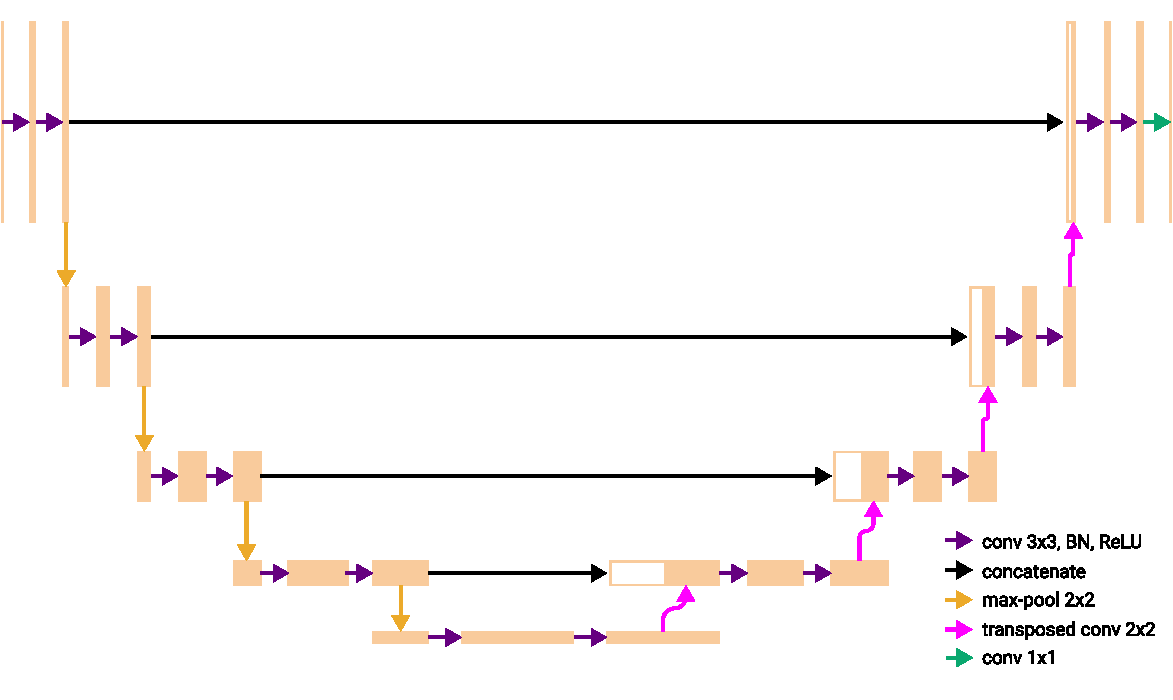
\includegraphics[width=0.8\linewidth]{figures/3_theoretical_background/deep learning/unet.pdf}
    \fignote{One should notice that the model layers ressemble a U. Adapted from \href{https://innolitics.com/articles/medical-image-segmentation-overview/}{Innolitics}}
    \label{fig:unet}
\end{figure}

Several variations of U-Net have been proposed over the years, such as U-Net++ and Attention U-Net, which introduce improvements in skip connections to increase the accuracy and efficiency of the model. In addition, there are also variations that change the encoder to classics \acs{CNN}s architectures such as ResNet or EfficientNet - without using the final \ac{MLP} (see Section \ref{sec:mlp}) - aiming to improve the model's feature extraction capability.


\subsubsection{AutoEncoder (AE)}

\Acf{AE} is a \ac{DL} architecture designed to learn compressed representations of input data, usually for dimensionality reduction or feature learning later used in another model \citep{hinton2006reducing}. An autoencoder consists of two main parts: the encoder and the decoder. The encoder maps the input data to a lower-dimensional latent space, compressing the information, while the decoder reconstructs the original data from this compressed representation (see Figure \ref{fig:autoencoder}).

\begin{figure}[ht!]
    \centering
    \caption{Diagram of a AutoEncoder model.}
    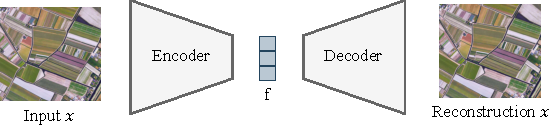
\includegraphics[width=0.85\linewidth]{figures/3_theoretical_background/deep learning/autoencoder.pdf}
    \fignote{Adapted from \href{https://uvadlc-notebooks.readthedocs.io/en/latest/tutorial_notebooks/tutorial9/AE_CIFAR10.html}{UvA Deep Learning Tutorials}}
    \label{fig:autoencoder}
\end{figure}

There are several types of autoencoders, including Denoising Autoencoders, which learn to reconstruct noisy data, and Variational Autoencoders (VAEs), which introduce a probabilistic approach to data generation - allowing, for example, the generation of data that mixes different classes. In \ac{RS}, autoencoders are often used for pretraining models, but this topic will be better addressed in Section \ref{sec:ssl_contextualization}.

\subsubsection{Generative Adversarial Network (GAN)}

\Acf{GAN} is a DL architecture composed of two neural models that compete with each other: the generator and the discriminator. The generator creates synthetic data from a random input, while the discriminator attempts to distinguish between real and generated data. During training, both models are trained, the generator learns to create increasingly realistic data, while the discriminator becomes more effective at identifying false data (see Figure \ref{fig:gan}). The convergence of this process is theoretically guaranteed by the ``Nash equilibrium'', in which both the generator and the discriminator have no significant gains in changing their strategy, although this is usually only seen approximately in practice.

\begin{figure}[ht!]
    \centering
    \caption{Diagram of a Generative Adversarial Network model.}
    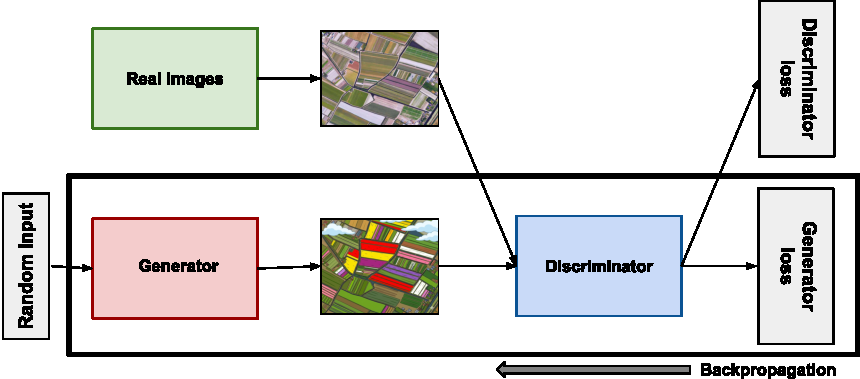
\includegraphics[width=1\linewidth]{figures/3_theoretical_background/deep learning/gan.pdf}
    \fignote{Adapted from \href{https://developers.google.com/machine-learning/gan/generator}{Google Developers}}
    \label{fig:gan}
\end{figure}

In \ac{RS}, \acs{GAN}s are used for various applications, such as synthetic image generation, image translation between different domains (e.g., from radar images to optical images), and especially for super-resolution of satellite images \citep{goodfellow2014generative}. In addition, \acs{GAN}s are also used to augment limited datasets by generating additional samples that help improve the performance of supervised models, which is useful for scenarios with very little data, as is often the case with Crop Yielding. However, \acs{GAN}s are known to potentially generate artifacts in the images they produce, which can be a challenge in applications that require high fidelity, in addition to the impossibility of auditing the generated data, making them difficult to use in applications such as deforestation Change Detection.


\subsubsection{Recurrent Neural Network (RNN)}
\label{sec:rnn}

A \ac{RNN} is a \ac{DL} model designed to handle sequential data, used in \ac{RS} for time series processing, whether pixels or images, through hybrid models with \ac{CNN}. \acs{RNN}s have recurrent connections that allow information from previous steps in the sequence to be retained and used to influence predictions in subsequent steps.

\acs{RNN}s work through a hidden state ($h_t$) that is updated at each step of the sequence ($x_t$), allowing the model to capture temporal dependencies in the data and produce an output ($y_t$) at each step (see Figure \ref{fig:rnn}). However, they suffer from the problem of gradient vanishing, which makes it difficult to learn long-term dependencies in long sequences.

\begin{figure}[ht!]
    \centering
    \caption{Diagram of a Recurrent Neural Network model.}
    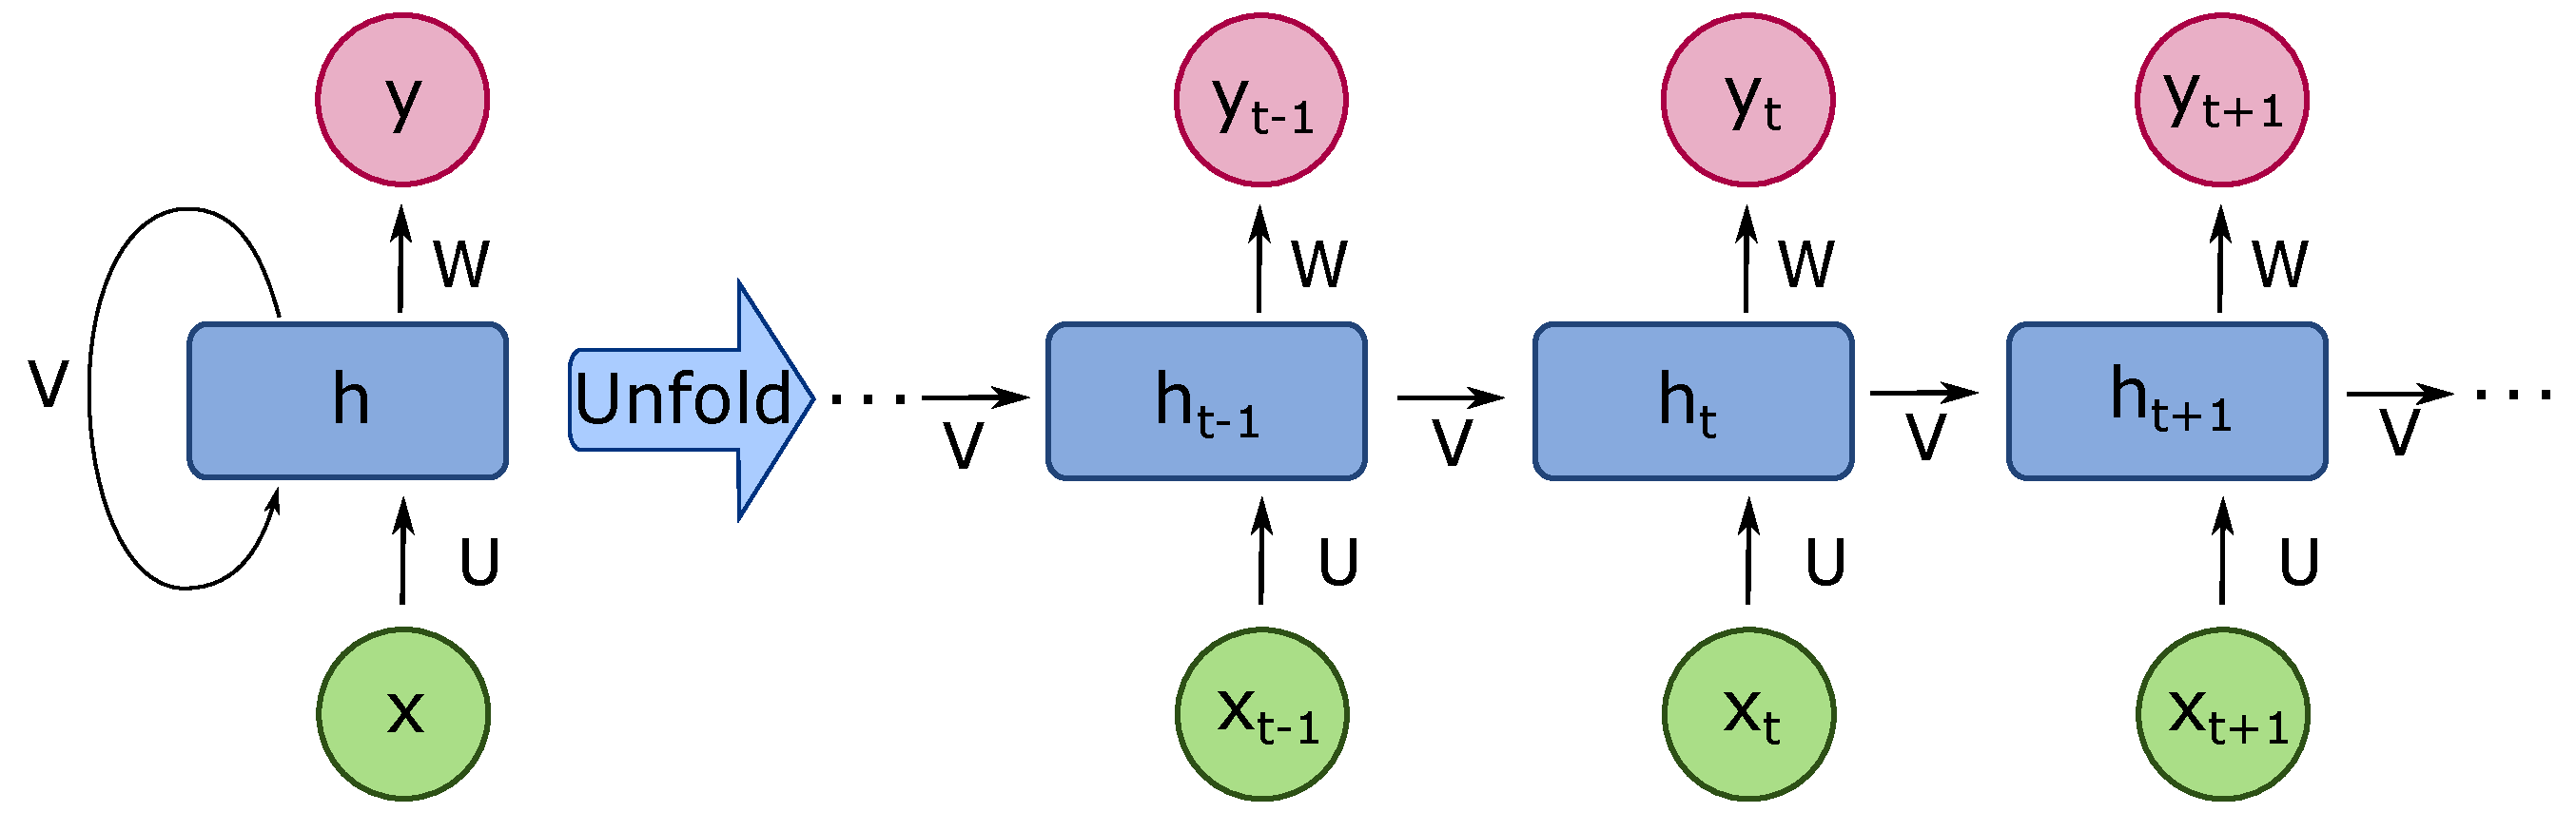
\includegraphics[width=.7\linewidth]{figures/3_theoretical_background/deep learning/rnn.pdf}
    \fignote{Adapted from \href{https://commons.wikimedia.org/wiki/File:Recurrent_neural_network_unfold.svg}{RNN - Wikimedia}}
    \label{fig:rnn}
\end{figure}

\subsubsection{Long Short-Term Memory (LSTM)}
\label{sec:lstm}

A \ac{LSTM} is an evolution of \ac{RNN} designed to mitigate vanishing gradients, allowing the model to capture long-term dependencies in sequential data \citep{graves2012long}. \acs{LSTM}s introduce a special cell structure (see Figure \ref{fig:lstm}) that includes input, forget, and output gates, allowing the model to control the flow of information and retain or discard information as needed.

\begin{figure}[ht!]
    \centering
    \caption{Diagarm of a Long Short-Term Memory model.}
    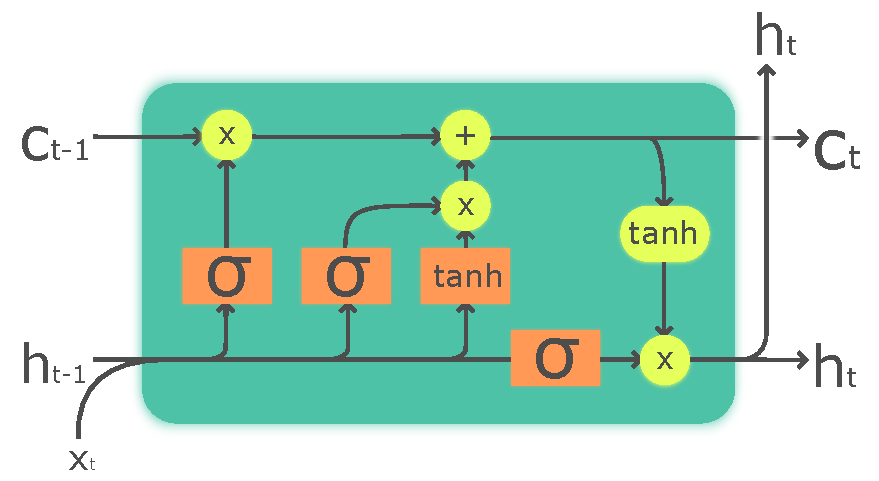
\includegraphics[width=.7\linewidth]{figures/3_theoretical_background/deep learning/lstm.pdf}
    \fignote{Adapted from \href{https://commons.wikimedia.org/wiki/File:The_LSTM_Cell.svg}{LSTM - Wikimedia}}
    \label{fig:lstm}
\end{figure}

The basis of the \ac{LSTM} is the cell state ($C_t$), a data line that runs through the entire chain and is protected by three gates that regulate what enters and what leaves. The Forget Gate ($\sigma$) decides, based on the current input ($x_t$) and the previous hidden state ($h_{t-1}$), which information from $C_{t-1}$ will be discarded or retained. Next, the Input Gate (composed of a Sigmoid $\sigma$ and a $\tanh$) determines which new data is important and adds it to the state cell. The new cell state ($C_t$) is then a combination of the old memory (filtered by the Forgetting Gate) and the new information (added by the Input Gate). Finally, the Output Gate ($\sigma$) decides which parts of $C_t$ (scaled by a tanh function) will be exposed as the hidden state ($h_t$) for the next time step, which is the actual output of the \ac{LSTM} unit to the subsequent layer and the next time step, completing the memory and prediction cycle.

A common variation of this architecture is the \acf{GRU}, which simplifies the LSTM by merging the forget and input gates into a single ``update gate'' and combining the cell state and hidden state \citep{cho2014learning}. This results in a more computationally efficient model with fewer parameters while maintaining similar performance in many tasks. Furthermore, the \acf{BiGRU} enhances this by processing the sequence in both forward and backward directions simultaneously \citep{schuster1997bidirectional}. This allows the model to capture context from both past and future states at any given time point, which is particularly useful for understanding the complete temporal evolution of a signal.

In \ac{RS}, \acs{LSTM}s and \acs{GRU}s have already been used for Crop Classification \citep{russwurm2023end} and Crop Yielding \citep{cheng2022wheat,jeong2022predicting}, due to the nature of time series in both applications. They are usually used pixel by pixel, i.e., each time series for each pixel is processed individually.

\subsubsection{Transformer}
\label{sec:transformer}

Transformer is a DL architecture originally developed for \acs{NLP}s tasks \citep{vaswani2017attention}, but which has been adapted for several other areas, including computer vision. This architecture has revolutionized the field of \ac{DL} due to its ability to capture long-range dependencies in sequential data, forming the basis for the construction of both commercial \acs{LLM}s such as ChatGPT \citep{openai2024gpt4technicalreport} and open source models such as Gemma \citep{gemmateam2025gemma3technicalreport}.

\begin{figure}[ht!]
    \centering
    \caption{Diagram of a Transformer model.}
    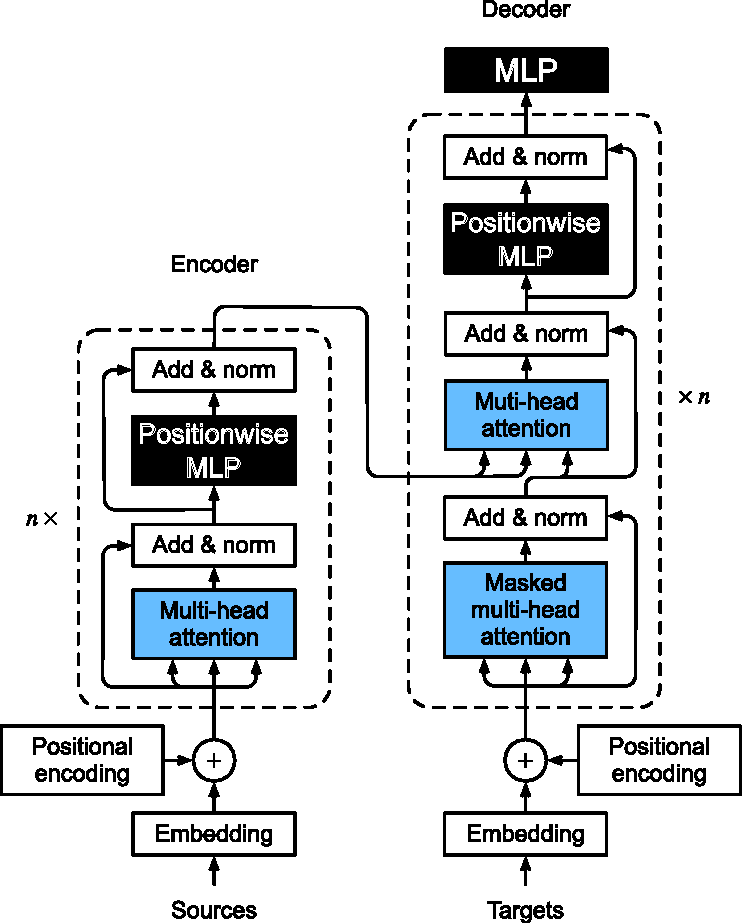
\includegraphics[width=0.7\linewidth]{figures/3_theoretical_background/deep learning/transformer.pdf}
    \fignote{Adapted from \href{https://pt.d2l.ai/chapter_attention-mechanisms/transformer.html/}{Dive into Deep Learning}}
    \label{fig:transformer}
\end{figure}

The model works by converting and processing data sequences through two interconnected structures, the Encoder (left) and the Decoder (right), which operate in $N$ repeated layers. The process begins by converting the inputs and targets into embeddings that are added (or concatenated, depending on the implementation) to a positional encoding to preserve the order of the elements. In the Encoder, Multi-head attention mechanisms simultaneously analyze the relationships between all parts of the input to create a rich representation of the context, which is refined by MLPs and normalizations for each point in the series. This contextualized representation is then sent to the Decoder, which combines the history of what has already been generated (using Masked multi-head attention to prevent access to future words) with the information coming from the Encoder, processing everything to generate the probability of the next output through a final \ac{CNN} (see graphically in Figure \ref{fig:transformer}).

Transformers were used in \ac{RS}, especially through some variations, such as the Vision Transformer (ViT) \citep{lin2023mmst} and the adapted \ac{BERT} \citep{shravan2024sits}, which will be explained later. In addition, the attention mechanism introduced by Transformers has been incorporated into several \ac{DL} architectures to improve the ability to capture spatial and temporal dependencies in \ac{RS} data.

\subsubsection{Vision Transformer (ViT)}

\Acf{ViT} is an adaptation of the Transformer architecture (see Setion \ref{sec:transformer}) for computer vision tasks such as image classification and semantic segmentation \citep{dosovitskiy2020image}. \ac{ViT} divides an image into small patches (e.g., $16\times16$ pixels), which are then flattened and transformed into embeddings, similar to words in \ac{NLP}. These embeddings are summed (or concatenated) with a positional encoding to preserve the spatial information of the patches before being fed into the Transformer model. The rest of the architecture follows the Transformer pattern, with Multi-head attention layers and \ac{MLP}s to process the embeddings of the patches and capture the relationships between them (see Figure \ref{fig:vit}), however, since the goal is not to generate a new image, the decoder is not used (which makes the architecture a subclass of Transformers called ``encoder-only'').


\begin{figure}[ht!]
    \centering
    \caption{Diagram of a Vision Transformer model.}
    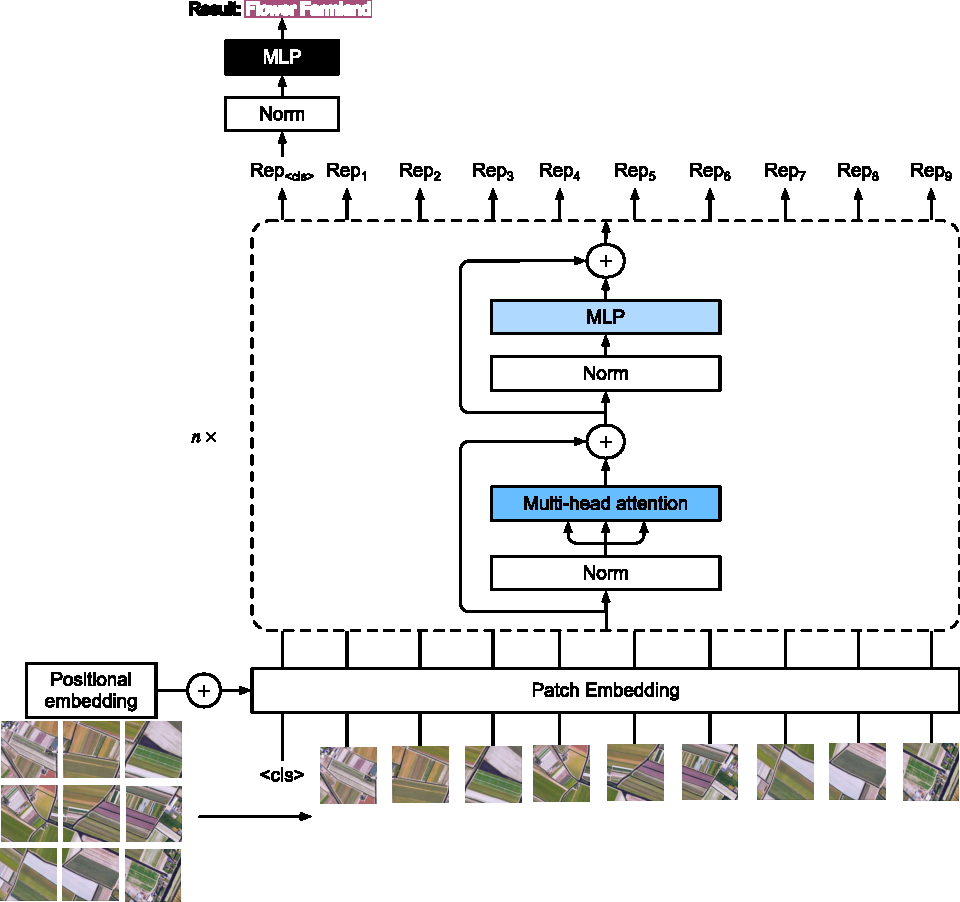
\includegraphics[width=0.7\linewidth]{figures/3_theoretical_background/deep learning/vit.pdf}
    \fignote{Adapted from \href{https://d2l.ai/chapter_attention-mechanisms-and-transformers/vision-transformer.html}{Dive into Deep Learning}}
    \label{fig:vit}
\end{figure}

Several variations of \ac{ViT} have been proposed, such as Swin Transformer, which introduces hierarchical attention mechanisms to improve the ability to capture features at different scales called Shifted windows, much like what \ac{CNN} do with their convolutional and pooling layers. The central idea is to subdivide the image several times, but each subdivision has its grid shifted relative to the previous one, allowing the model to capture both local and global features efficiently. A variation widely used in \ac{RS} is SwinNet, which combines the Swin Transformer as an encoder with an \ac{FCN}-based decoder (see Section \ref{sec:fcn}) to perform semantic segmentation.

\subsubsection{Bidirectional Encoder Representations from Transformers (BERT)}

\Acf{BERT} is a \ac{DL} model based on the Transformer architecture (see Section \ref{sec:transformer}) designed for NLP tasks \citep{devlin2019bert}. \ac{BERT} is trained using an unsupervised pre-training approach, where the model learns to predict masked words in a sentence (Masked Language Modeling) and to predict the next sentence in a pair of sentences (Next Sentence Prediction). It is known that predicting the next word is not necessary \citep{liu2019roberta}. This approach allows \ac{BERT} to capture the bidirectional context of words, considering both the context to the left and right of a word in a sentence. Subsequently, the model can be fine-tuned for a specific task, such as grammatical classification using less labeled data (see Figure \ref{fig:bert}). Note that details about \ac{SSL} pre-training, which is the case with BERT, will be better addressed in Section \ref{sec:ssl_contextualization} (the BERT pre-training, which is a Masked Modeling pre-training, it is discussed in details in Section \ref{sec:ssl_mim}).

\begin{figure}[ht!]
    \centering
    \caption{Diagram of a Bidirectional Encoder Representations from Transformers model.}
    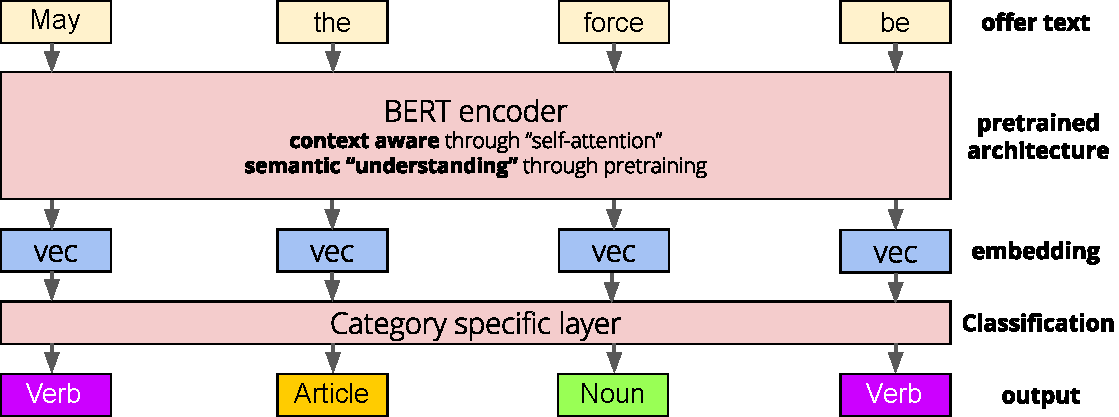
\includegraphics[width=.85\linewidth]{figures/3_theoretical_background/deep learning/bert.pdf}
    \fignote{Adapted from \href{https://dida.do/projects/numeric-attribute-extraction-from-product-descriptions}{Dida.do}}
    \label{fig:bert}
\end{figure}

Although \ac{BERT} was designed to handle \ac{NLP} data, its basic idea of Bidirectional Encoder has been adapted for other purposes such as DNA analysis \citep{zhou2025dnabert}, protein analysis \citep{brandes2022proteinbert}, and item recommendation \cite{sun2019bert4rec}. In Remote Sensing, variations of \ac{BERT} have been adapted to process \ac{SITS}, using spectral bands linearly projected directly into the \ac{BERT} Encoder.

\subsubsection{Mamba and the post-Transformer question}

Although Transformers (see Section \ref{sec:transformer}) have established the state of the art in several tasks, their architecture presents a fundamental limitation: the computational and memory complexity of the self-attention mechanism scales quadratically ($O(L^2)$) with respect to the sequence length $L$. There are even ethical discussions about the environmental impacts caused by LLMs, which almost entirely use Transformers. Which model performs as well as a Transformer but is linear ($(O(L))$) or linear-logarithmic ($(O(L\times \log L))$) is perhaps the major current question in the field of Machine Learning, with the other major question being whether such a model can even exist.

One attempt to address this is through state-space models (SSMs), with the Mamba model as its main representative. Mamba introduces a selection mechanism that allows the model to filter out irrelevant information and focus on specific contextual data, operating with linear complexity ($O(L)$).

\begin{figure}[ht!]
    \centering
    \caption{Diagram of a Mamba model.}
    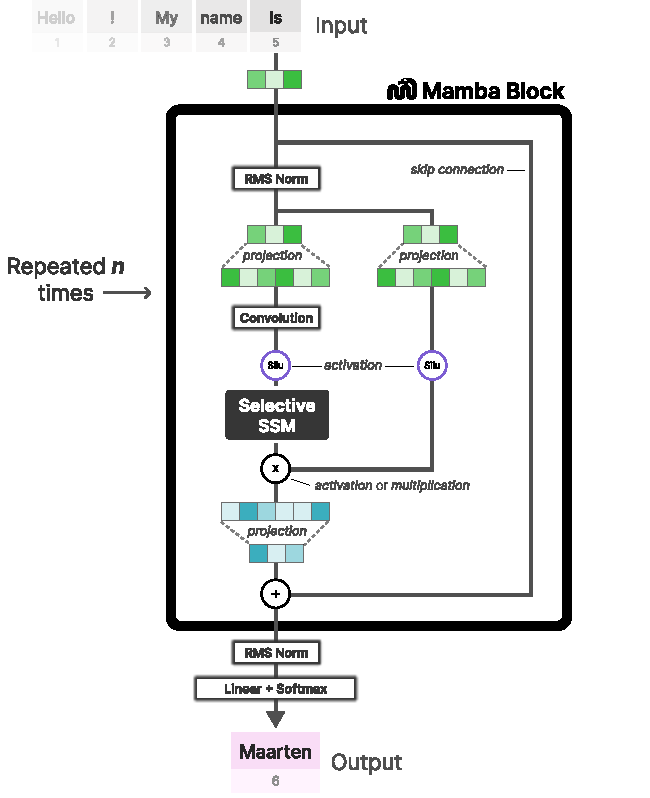
\includegraphics[width=0.75\linewidth]{figures/3_theoretical_background/deep learning/mamba.pdf}
    \fignote{Adapted from \href{https://www.maartengrootendorst.com/blog/mamba/}{
Maarten Grootendorst Blog}}
    \label{fig:mamba}
\end{figure}

The Mamba architecture is based on Selective State Space Models (S6), which allow model parameters to be functions of the input, giving it a contextual reasoning capability comparable to that of Transformers. In the field of computer vision, this approach gave rise to Vision Mamba (Vim) \citep{zhu2024vision} and VMamba \citep{liu2024vmamba}, which adapt linear scanning to two-dimensional data through the Cross-Scan Module, allowing the model to capture spatial dependencies in images without the high cost of global attention.